\scanpage{61}
\mspage{17}
Recapitulation of the elementary operations

\inserted{$(0^\circ)$ Disjoint sum}

$\unsure{4^\circ|1^\circ}$) \uline{erasure} \inserted{of \uline{all} the marks at $a$, i.e.} of the marks lying on a circle \inserted{\unsure{$C_a$|$C_0$}} for gluing \inserted{\unsure{the|$C_a$}}, or \deleted{\unsure{on a circle}} for cutting
$\Longleftrightarrow$ removal \unsure{of a|of the} \deleted{part} \inserted{$R_a$}
$(a\in A)$ $\Longleftrightarrow$ modification of $\underline r$ by
\deleted{\unsure{of $R$ lying in a part}}
replacing it by $0$ at $a$.
\margin{\uline{strongly}\\\uline{irreversible}\\ $r_a\ne0$}

$2^\circ$) \inserted{\uline{uniform partial} \uline{erasure}: \uline{of exponent $d_a\mathrel{:\!|}r_a$}}
Restriction of the \deleted{scalars} \inserted{groups of $R_a$} from $\mathbb Z_a/r_a\mathbb Z$ to a
$\mathbb Z_a/r'_a\mathbb Z_a$, where $r'_a\mid r_a$ \raisebox{-.4ex}{\unsure{2|?}}
(for fixed $a$, there are $r_a/r'_a=d_a$ possible choices, where we assume $d_a>1$ i.e. $r'_a\ne r_a$).
\margin{%
\begin{tikzpicture}[baseline=(m2label.base)]
\node[anchor=north west,inner sep=1pt,align=left] (m2label) at (0,0)
 {\uline{strengthening} \unsure{of|of the}\\\uline{\unsure{weak|weak} \unsure{structure|structures}}\\$r_a\unsure{\ge|>}1$};
\draw ([xshift=-1pt,yshift=3pt]m2label.north west) --
 ([xshift=3pt,yshift=3pt]m2label.north east) --
 ([xshift=3pt]m2label.south east);
\node[anchor=north west,inner sep=1pt,align=left] at ([yshift=-3pt]m2label.south west)
 {\deleted{\unsure{anodyne}}\\
 $r'_a\unsure{\mid|\ne}r_a$ and $r'_a\ne r_a$\\
 i.e. $d_a=\dfrac{r_a}{r'_a}\ne1$};
\end{tikzpicture}}

$3^\circ$) \deleted{Extension of the}
\inserted{\uline{uniform \unsure{-erasure|un-erasure}} \uline{of exponent} $d_a>1$}
--- i.e. extension of the groups of $R_a$ from
$\mathbb Z_a/r_a\mathbb Z_a$ to $\mathbb Z/\unsure{d|d_a}r_a\mathbb Z$,
\margin{%
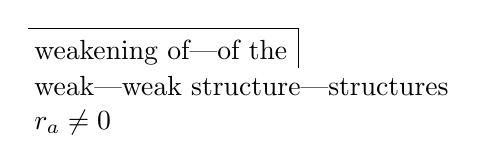
\begin{tikzpicture}[baseline=(m3label.base)]
\node[anchor=north west,inner sep=1pt,align=left] (m3label) at (0,0)
 {\uline{weakening \unsure{of|of the}}};
\draw ([xshift=-1pt,yshift=3pt]m3label.north west) --
 ([xshift=3pt,yshift=3pt]m3label.north east) --
 ([xshift=3pt]m3label.south east);
\node[anchor=north west,inner sep=1pt,align=left] at ([yshift=-2pt]m3label.south west)
 {\uline{\unsure{weak|weak}} \unsure{structure|structures}\\$r_a\ne0$};
\end{tikzpicture}}

\margin{\rule{2cm}{.3pt}\\strongly irreversible}
\noindent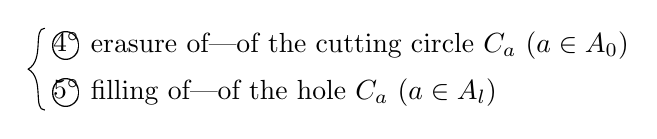
\begin{tikzpicture}[baseline=(ops.center)]
\node[anchor=west,inner sep=0pt,align=left] (ops) at (0,0)
 {\begin{tabular}{@{}l@{}}
 \textcircled{$4^\circ$} erasure \unsure{of|of the} cutting circle $C_a$ $(a\in A_0)$\\[1.2ex]
 \textcircled{$5^\circ$} filling \unsure{of|of the} hole $C_a$ $(a\in A_l)$
 \end{tabular}};
\draw ([xshift=-.2em]ops.north west)
 .. controls ([xshift=-.65em]ops.north west) and ([xshift=-.2em,yshift=.35em]ops.west)
 .. ([xshift=-.8em]ops.west)
 .. controls ([xshift=-.2em,yshift=-.35em]ops.west) and ([xshift=-.65em]ops.south west)
 .. ([xshift=-.2em]ops.south west);
\end{tikzpicture}

$6^\circ$) Cutting along $C_a$ $(a\in A_0)$ \({}^*\)
\margin{\rule{2cm}{.3pt}\\strongly irreversible if $r_a=0$, \deleted{\unsure{weakly|weak}} reversible = anodyne if $r_a\ge1$.}

$7^\circ$) Gluing along $C_a,C_{a'}$
(\unsure{with} $a,a'\in A_l$, $a\ne a'$, \inserted{$r_a=r_{a'}$}), via an element of
$R_a\mathbin{\wedge}R_{a'}$.
\margin{\rule{2cm}{.3pt}\\$r_a=r_{a'}\unsure{\ge|>}1$\quad reversible = anodyne}

\margin{--- \({}^*\) One should \inserted{perhaps} split $6^\circ)$ in two, according as $r_a=0$ or $r_a\ne0$ (or \unsure{$=$|\deleted{or}} exclude the case $r_a=0$?)}
\mspage{60}
